\section{Développement de l'application}

\indent L'application finale demandée reprend les éléments de configuration vus en section 2.
Cette section comporte un récapitulatif des éléments de l'application avec éventuellement des portions de code montrant leur utilisation.
Un exemple de résultats obtenus après lancement de l'application sont montrés.

\subsection{Cahier des charges}

\indent Il s'agit d'implanter une application simple permettant de mesurer le temps de réaction d'une personne (Utilisateur) et mettant en œuvre différentes entrées/sorties disponibles sur la carte SAMD21 en utilisant SW0 et LED0 et sur la carte OLED1 (extension de la carte SAMD21) en utilisant BP1, BP2, BP3, LED1, LED2, LED3 et l'écran OLED.
La structure fonctionnelle de l'application à développer peut être présentée dans un premier temps (légèrement modifiée par la suite) par la figure suivante :

\begin{figure}[h]
    \centering
    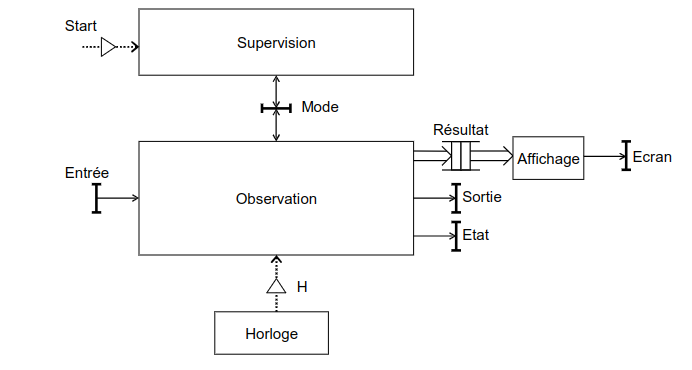
\includegraphics[width=0.7\linewidth]{struct_fonc.png}
    \caption{Structure fonctionnelle initiale de l'application à développer}
    \label{fig:struct}
\end{figure}

\indent La mesure de vitesse de réaction est démarrée lors de l'apparition de l'événement Start.
Elle consiste alors à émettre un code aléatoire en allumant un ensemble de LED (variable Sortie matérialisée par LED1, LED2 et LED3) et à mesurer le temps nécessaire à l'utilisateur pour reproduire la combinaison sur des boutons poussoirs (variable Entrée, matérialisée par BP1, BP2 et BP3) en comptant le nombre d'événements H entre la production d'une valeur sur Sortie et la reproduction de cette valeur sur Entrée. 
Plusieurs mesures de vitesse de réaction peuvent être effectuées afin d'obtenir des valeurs minimale, moyenne et maximale (constante NbMesToDo dans l'automate présenté par la suite, constante dont la valeur est strictement supérieure à 1, peut avoir la valeur 5 par exemple).
Lorsque toutes les mesures ont été effectuées, des statistiques sont transmises à la fonction Affichage qui se charge de les afficher sur l'Ecran de la carte OLED1.
La précision de la mesure du temps de réaction doit être de 1 ms.
L'état de la fonction d'observation (Observe ou Non\_Observe) est en permanence affiché (variable Etat, matérialisée par LED0 de la carte SAMD21XPLAINEDPRO, la LED0 doit être allumée lorsqu'Etat a la valeur Observe).
Le comportement de la fonction Observation est défini par l'automate de la figure \ref{fig:automate}.


\subsection{Éléments de l'application}

L'application se base sur la structure fonctionnelle suivante :

\begin{figure}[h]
    \centering
    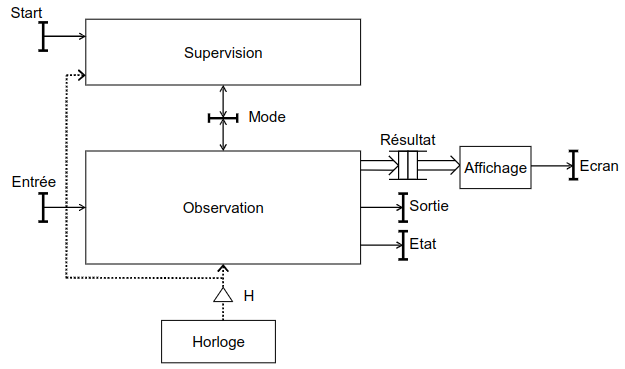
\includegraphics[width=0.7\linewidth]{struct_fonc_final.png}
    \caption{Structure fonctionnelle de l'application à développer}
    \label{fig:struct_final}
\end{figure}

\indent Par rapport à la structure fonctionnelle présentée en figure \ref{fig:struct}, \textit{Start} n'est plus un évènement mais une variable partagée.
Cette solution est plus simple à implanter car elle ne nécessite pas la gestion des interruptions engendrée par l'attente d'un évènement en entrée du système.
De ce schéma, différentes informations peuvent être extraites.
Quatre tâches distinctes peuvent être imaginées pour cette application temps-réel:

\begin{itemize}
    \item Horloge
    \item Supervision
    \item Observation    
    \item Affichage
\end{itemize}

\indent Il peut être fait l'hypothèse que deux sémaphores, matérialisées dans la structure par l'évènement H en entrée des tâches "Supervision" et "Observation", peuvent être implantées au sein de l'application.
L'application contient une variable partagée \textit{Mode} et une file de message \textit{Résultats}.
Les différentes entrées/sorties présentées dans cette structure fonctionnelle correspondent à des éléments physiques présents sur la carte tels que des boutons poussoirs, des LEDs ou l'écran.

\subsection{Code de l'application}

\indent L'application a été développée sur l'environnement Microchip Studio.
Cet environnement est adapté au développement d'une application temps-réel et nécessite deux cibles: une machine de développement et une cible.
Il est en effet équipé d'une chaîne de cross-compilation et peut programmer la cible via une liaison série.
Il est également équipé d'un outil de debug.
Dans le cadre du projet, la cible est une carte SAMD21XPLAINEDPRO et sa carte d'extension OLED1XPLAINEDPRO.
La cible recevra l'application tournant sur un exécutif temps-réel FreeRTOS.\\
\indent Au long des séances de projet, l'exécutif temps-réel FreeRTOS a été configuré de sorte à pouvoir recevoir l'application.
Il est par exemple possible, via modification du fichier FreeRTOSConfig.h, de modifier l'horloge de référence du CPU reçue par FreeRTOS.
Dans le cadre du projet, l'horloge de référence a une fréquence de 8 MHz.
De plus, il est possible de définir le nombre de Ticks d'horloge par seconde envoyé par FreeRTOS aux applications.
Ici, l'OS envoie 1000 Ticks/secondes soit une fréquence de 1 kHz.
La gestion des horloges au sein du système peut être résumée ainsi:

\begin{figure}[h]
    \centering
    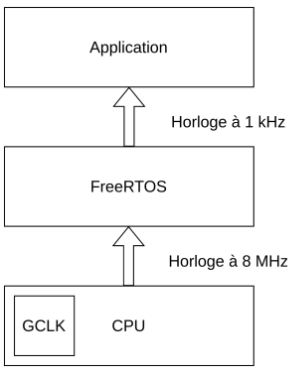
\includegraphics[width=0.7\linewidth]{horloges.png}
    \caption{Configuration des horloges pour l'application}
    \label{fig:clock}
\end{figure}

\indent Enfin, il est possible de modifier la taille de pile allouée à l'application.
Par défaut cette taille est de 60.
Progressivement, au fil des séances, des éléments ont été ajouté à l'application, notamment la gestion de l'écran OLED.
Une profondeur de pile de 60 n'est pas suffisante suite à l'ajout de l'écran; cette taille doit être réajustée.
Pour la suite du projet, la taille a été définie à 100.
Cette taille n'a pas été raffinée, mais en vue d'obtenir une application plus performante, la taille minimale nécessaire pourrait être trouvée.\\
\indent L'application en elle même contient la définition des quatre tâches vues précédemment, des variables globales, des variables partagées, des sémaphores et de la file de message.
Les différents éléments sont crées et l'ordonnanceur est démarré dans la fonction \textit{main()}.
Chaque tâche a une priorité qui lui est propre et un comportement précisé dans le corps du sujet.
Dans un premier temps, le comportement de chaque tâche sera défini en accordance avec la structure fonctionnelle (figure \ref{fig:struct_final}).
\\\\
\textbf{Horloge}
\\\\
La tâche Horloge est responsable de l'envoi des deux sémaphores de l'application. 
Elle envoie un sémaphore d'éveil \textit{H1} à la tâche Observation et un sémaphore d'éveil \textit{H2} à la tâche Supervision.
Au préalable, elle contient un appel à la procédure vTaskDelay qui correspond à un temps d'attente d'un certain nombre de Tick d'horloge.
Par défaut, ce nombre est défini à 1 et ne changera pas pour la suite du projet.
\\\\
\textbf{Observation}
\\\\
La tâche Observation est éveillé par le sémaphore \textit{H1} en provenance de la tâche Horloge.
Cette tâche a un comportement donné par l'automate suivant:

\begin{figure}[h]
    \centering
    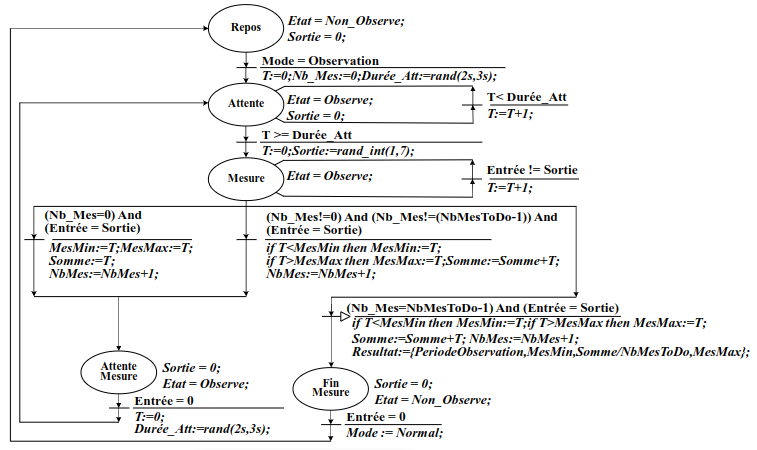
\includegraphics[width=0.9\linewidth]{automate_obs.png}
    \caption{Automate de la tâche Observation}
    \label{fig:automate}
\end{figure}

\indent La tâche Observation effectue les mesures du temps de réaction.
Pour démarrer une série de mesures, l'état de la variable partagée \textit{mode} est testé dans l'état initial de repos.
L'état de la variable partagée est modifié dans la tâche Supervision.
Lorsque \textit{mode} est égale à Observation, la série de mesures démarre.
A chaque mesure, selon que ce soit la première, une mesure au milieu de la série ou une mesure de fin, le comportement souhaité n'est pas le même.
Lors de la dernière mesure, les prises de mesures sont finies et envoyées via une file de message Résultats à la tâche Affichage.
\\\\
\textbf{Supervision}
\\\\
La tâche Supervision est, comme la tâche Observation, éveillé par un sémaphore en provenance de la tâche Horloge.
Cette tâche écrit sur la variable partagée \textit{mode} lorsque le bouton BP0 est appuyé, permettant de démarrer l'application.
L'algorithme donné de la tâche observation est le suivant:

\begin{figure}[h]
    \centering
    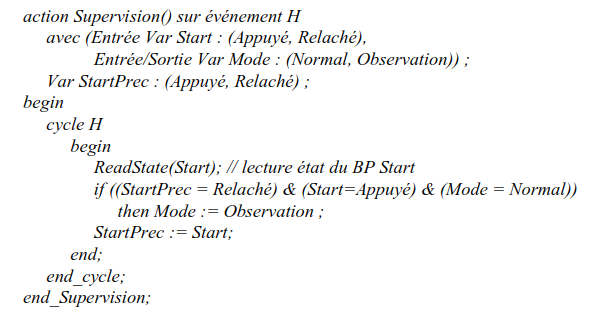
\includegraphics[width=0.7\linewidth]{algo.png}
    \caption{Algorithme de la tâche Supervision}
    \label{fig:algo}
\end{figure}

\textbf{Affichage}
\\\\
La tâche Affichage est activée sur réception de la file de message Résultats en provenance de la tâche Observation.
Les résultats sont lus puis affichés sur l'écran.
\\\\

\indent Les quatres tâches décortiquées ci-dessus nécessitent d'avoir des priorités définies.
Selon la politique d'ordonnancement de FreeRTOS (\ref{ordonnancement}), les tâches sont exécutées selon l'ordre de priorité le plus élevé.
Dans le cadre de l'application développé, les priorités de chaque tâche sont définies ainsi:

\begin{lstlisting}[style=CStyle]
    #define CLOCK_TASK_PRIORITY ( tskIDLE_PRIORITY +5 ) 
    #define OBSERVATION_TASK_PRIORITY ( tskIDLE_PRIORITY +2 )
    #define SUPERVISION_TASK_PRIORITY ( tskIDLE_PRIORITY +3 )
    #define AFFICHAGE_TASK_PRIORITY ( tskIDLE_PRIORITY +1 )
\end{lstlisting}

\indent La tâche la plus prioritaire est logiquement l'horloge puisqu'elle envoie les sémaphores nécessaires à l'éveil des autres tâches.
La tâche Supervision est plus prioritaire que la tâche Observation puisqu'elle écrit sur la variable partagée \textit{mode} qui est lue dans la tâche Observation.
Enfin, la tâche Affichage est la moins prioritaire puisqu'elle reçoit une file de message de la tâche Observation.

\subsection{Résultat}

L'application peut être testée en programmant la carte.
L'utilisateur doit appuyer sur le bouton SW0 pour lancer une série de mesures du temps de réaction.
Dans le cadre des résultats montrés ci-dessous, cinq mesures successives sont effectuées avant l'affichage des résultats sur l'écran.
Les figures suivantes montrent l'affichage de l'écran au lancement de l'application (figure \ref{fig:start_app}) et à la fin d'une série de mesure (figure \ref{fig:end_app}).
Les résultats montrés sont, dans l'ordre:

\begin{itemize}
    \item Le temps de réaction minimal
    \item Le temps de réaction moyen
    \item Le temps de réaction maximal
    \item La période d'observation entre deux appels de la tâche Observation
\end{itemize}

L'unité de chacune de ces valeurs est le \textit{tick d'horloge}.
Le projet utilise une horloge à la fréquence de 8 MHz, divisée par un facteur AAA.
Ainsi, un \textit{tick d'horloge} correspond à approximativement BBB secondes.

\begin{figure}[h]
    \centering
    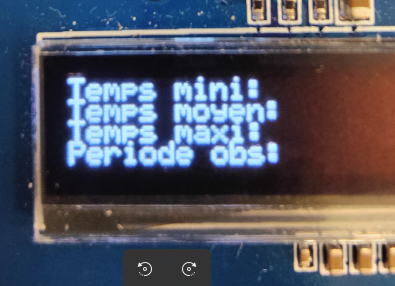
\includegraphics[width=0.4\linewidth]{start_app.png}
    \caption{Affichage de l'écran au lancement de l'application}
    \label{fig:start_app}
\end{figure}

Au lancement de l'application, l'écran affiche du texte en préparation de l'arrivée des résultats.
C'est lors de l'initialisation du matériel que cet affichage a lieu.

\begin{figure}[h]
    \centering
    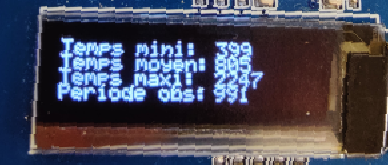
\includegraphics[width=0.4\linewidth]{end_app.png}
    \caption{Affichage de l'écran après une session de mesure du temps de réaction}
    \label{fig:end_app}
\end{figure}

\indent Après une série de mesures, la file de message contenant les résultats est envoyée de la tâche \textit{Observation} à la tâche \textit{Affichage}.
Cette file de message contient la variable Résultat, instance de la structure \textit{Resultat\_t} contenant les différentes mesures.
Après réception de la file de message, la tâche \textit{Affichage} fait apparaître sur l'écran les résultats de la mesure.
\\
\indent Pour prouver le bon fonctionnement de l'application, une vidéo est proposée dans le même dossier que ce rapport.
Cette vidéo couvre le démarrage de l'application après un reset. 
Une série de mesures a lieu, menant à l'affichage des résultats.
Enfin, l'utilisateur relance une série de mesures après appui sur le bouton SW0.
\\\\
\indent Outre l'aspet fonctionnel de l'application, il est nécessaire de prouver son bon fonctionnement d'un point de vue temps-réel.
La mesure de la période d'obsevation permet de justifier que les tâches s'exécutent dans une fenêtre de temps qui respecte les contraintes temporelles.
La tâche "Observation" est réveillée par une sémaphore en provenance de la tâche "Clock".
Selon la configuration du projet, l'horloge définie par l'OS pour les applications est de 1 khHz.
La tâche "Clock" envoie une sémaphore d'éveil après une attente de 1 Tick d'horloge.
La tâche "Observation" devrait donc être réveillée environ tout les 1000 Ticks d'horloge.
Lors des tests effectués, c'est ce qui a pu être observé, avec une valeur de période d'observation toujours comprise entre 990 et 994.
Dans le cas des résultats présentés en figure \ref{fig:end_app}, la période d'observation est de 991 Ticks d'horloge.